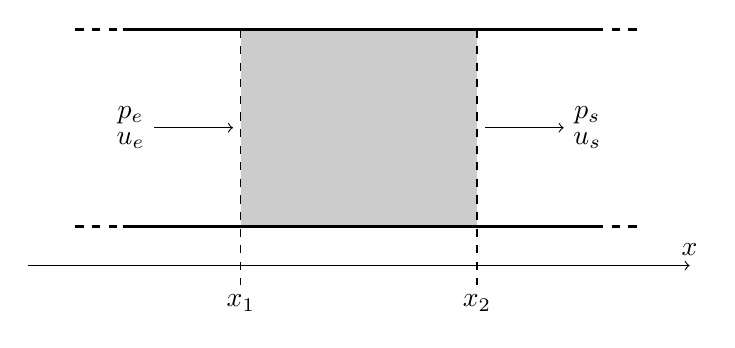
\begin{tikzpicture}
    \def\height{2.5};
    \def\length{6};
    \def\xone{\length/4};
    \def\xtwo{3*\length/4};
    \def\arrow{1};
    \def\xdist{9cm};
    
    \fill[black!20] (\xone,\height) rectangle (\xtwo,0);
    \draw[dashed] (\xone,\height) -- ++(0,-1.3*\height) node[below]{$x_1$};
    \draw[dashed] (\xtwo,\height) -- ++(0,-1.3*\height)node[below]{$x_2$};
    
    \draw[very thick,dashed] (-.1*\length,0) -- ++(.1*\length,0) coordinate(a1);
    \draw[very thick] (a1) -- ++(\length,0) coordinate(b1);
    \draw[very thick,dashed] (b1) -- ++(.1*\length,0);    
    \draw[very thick,dashed] (-.1*\length,\height) -- ++(.1*\length,0) coordinate(a2);
    \draw[very thick] (a2) -- ++(\length,0) coordinate(b2);
    \draw[very thick,dashed] (b2) -- ++(.1*\length,0);  
    
    \draw[<-] (\xone-.1,\height/2) -- ++(-\arrow,0) node[left]{\shortstack{$p_e$\\$u_e$}};
    \draw[->] (\xtwo+.1,\height/2) -- ++(+\arrow,0) node[right]{\shortstack{$p_s$\\$u_s$}};
    
    \draw[->] (-.2*\length,-.2*\height) --   ++(1.4*\length,0) node[above]{$x$};
    
%    \draw (a2) node[above]{\bf (a)};
    
    %%%%%
%    \begin{scope}[xshift=\xdist]
%    \fill[black!20] (\xone,\height) rectangle (\xtwo,0);
%    \draw[dashed] (\xone,\height) -- ++(0,-1.3*\height) node[below]{$x_1$};
%    \draw[dashed] (\xtwo,\height) -- ++(0,-1.3*\height)node[below]{$x_2$};
%    
%    \draw[very thick,dashed] (-.1*\length,0) -- ++(.1*\length,0) coordinate(a1);
%    \draw[very thick] (a1) -- ++(\length,0) coordinate(b1);
%    \draw[very thick,dashed] (b1) -- ++(.1*\length,0);    
%    \draw[very thick,dashed] (-.1*\length,\height) -- ++(.1*\length,0) coordinate(a2);
%    \draw[very thick] (a2) -- ++(\length,0) coordinate(b2);
%    \draw[very thick,dashed] (b2) -- ++(.1*\length,0);  
%    
%    \draw[->] (\xone-.1,\height/3) -- ++(-\arrow,0) node[midway,below]{$p_1^-$};
%    \draw[<-] (\xone-.1,2*\height/3) -- ++(-\arrow,0) node[midway,above]{$p_1^+$};
%    \draw[<-] (\xtwo+.1,\height/3) -- ++(+\arrow,0) node[midway,below]{$p_2^-$};
%    \draw[->] (\xtwo+.1,2*\height/3) -- ++(+\arrow,0) node[midway,above]{$p_2^+$};
%    
%    \draw[->] (-.2*\length,-.2*\height) --   ++(1.4*\length,0) node[above]{$x$};
%    
%    \draw (a2) node[above]{\bf (b)};
%    
%    \end{scope}
\end{tikzpicture}